\documentclass[letterpaper]{article} % Feel free to change this
\usepackage[utf8]{inputenc}
\usepackage{amsmath}
\usepackage{amsfonts}
\usepackage[english]{babel}
\usepackage{geometry}
\usepackage{mathtools}
\usepackage{parskip}
\usepackage{listings}

\topmargin=-0.45in
\evensidemargin=0in
\oddsidemargin=0in
\textwidth=6.5in
\textheight=9.0in
\headsep=0.25in

\begin{document}

\title{ECE 350: Digital Systems Project Checkpoint 4}
\author{Gordon Huynh} % Change this to your name
\date{\today} % Change this to the date you are submitting
\maketitle

\section*{Duke Community Standard}

By submitting this \LaTeX{} document, I affirm that
\begin{enumerate}
    \item I understand that each \texttt{git} commit I create in this repository is a submission
    \item I affirm that each submission complies with the Duke Community Standard and the guidelines set forth for this assignment
    \item I further acknowledge that any content not included in this commit under the version control system cannot be considered as a part of my submission.
    \item Finally, I understand that a submission is considered submitted when it has been pushed to the server.
\end{enumerate}

\newpage

\section*{Introduction}

This checkpoint contains a functional MIPS processor that implements hardware level interlocks. It is a 5-staged pipeline with specific stalls, bypasses, and flushing features to process MIPS instructions without any compiler inserted noops and such. It adheres to the ECE 350 ISA that involves various arithmetic instructions such as add, sub, lls; and various flow control instructions such as j, bne, jal, jr. Also specified by the ECE 350 spec sheet, the processor is built in a 32-bit architecture with 12-bit wide addresses. The processor reads instructions from ROM and is able to store persistent data in RAM or temporary data in its 32 32-bit registers. The core modules involved with this processor are the regfile, ALU, Mult/Div, and Latches.

\section*{Subcomponents}

\subsection*{Regfile}

The regfile is comprised of 32 32-bit registers. Each register is formed from 32 dflipflops. The input is split to every single register, but only the register specified by a control input will be allowed to persist the input. Data is updated every positive edge of the input clock and thus after a positive edge, new data should be available if a register was recently written too. As side feature, the regfile will also bypass new data to its output if the same register is being written and read from. All the outputs from the registers are wired to a tri-state buffer where it will output its signal if a control input specifies it. Otherwise, it will only provide a high-impedence.

\begin{figure}[htb!]
    \centering
    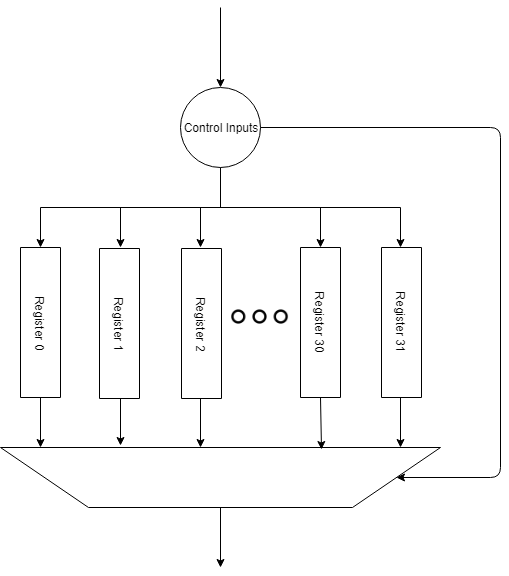
\includegraphics[width=.35\textwidth]{regfileDiagram.png}
    \caption{Design Diagram of Regfile}
\end{figure}

\newpage

\subsection*{ALU}

The main component to the ALU is the 32-bit adder. Specifically, the adder is implemented with a hierarchical carry-lookahead adder. The adder has 4 8-bit CLA adder blocks that each sum its given inputs. It outputs the sum, carryout, and the propagating and generating bit of its block. These bits are then used as the carry in for the next block. To perform subtraction, the ALU flips the sign of the second operand and adds them. For AND and OR, the ALU performs a bitwise operation on the inputs to reach the correct output. For arithmetic and logical shift, the ALU utilizes a barrel shifter where the operand is an input to a shifter of a set amount that is of base 2 (e.g. 1, 2, 4, 16). This output is multiplexed with its value before the shift and depending on the input shift amount, the shifted or unshifted value will continue. All of these operations occur simultaneously and the final result is multiplexed with a given opcode.

\begin{figure}[htb!]
    \centering
    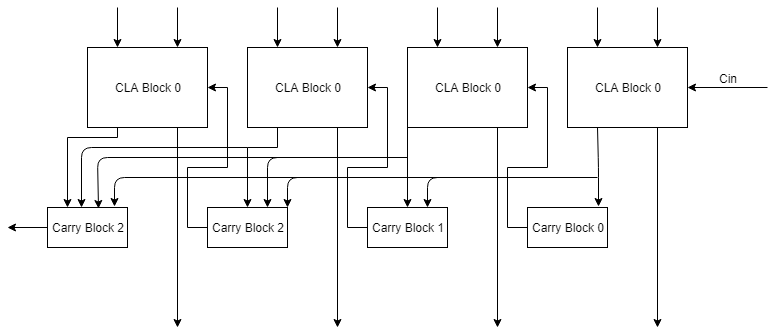
\includegraphics[width=.35\textwidth]{claAdderDiagram.png}
    \caption{Design Diagram of Hierarchical CLA Adder}
\end{figure}

\begin{figure}[htb!]
    \centering
    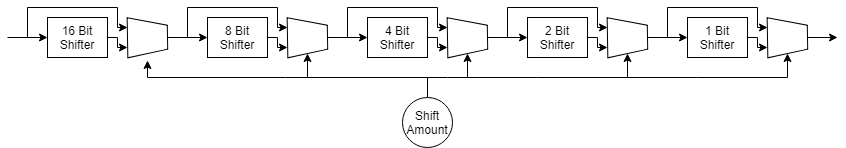
\includegraphics[width=.6\textwidth]{shifterDiagram.png}
    \caption{Design Diagram of Shifter}
\end{figure}

\subsection*{Mult/Div}
The multiplier is implemented with Booth's algorithm. It uses a 64 bit register to hold the initial multiplicand and the overall summation of the multiplication operation. The multiplicand is stored in the lower 32 bits. From Booth's we then add or subtract the multiplier from the higher half of the register. Then we shift the register right 1 and keep the bit that was removed to continue Booth's. We continue this process for 32 cycles and output the lower half of the register. The counter implemented is made of 33 dflipflops that outputs into the input of its neighbor. In this regard, whenever we start an operation, we assert the input of the first dflipflop. After 32 cycles, the last flip flop would output high to signal the end of an operation. For division, we again utilize a 64 bit register. The dividend is initially stored in the lower half of the register. Then the register is shifted left. If the divisor is less than whatever is in the upper half of the register, then we will append a 1 to the register on the next shift otherwise we append a 0. If we do append a 1, we then subtract the divisor from the upper half of the register. We continue this for 32 cycles then output the lower half of the register.

\newpage

\begin{figure}[htb!]
    \centering
    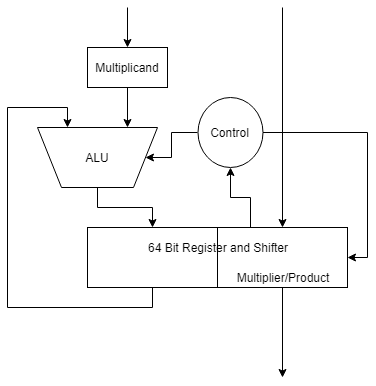
\includegraphics[width=.35\textwidth]{multiplierDiagram.png}
    \caption{Design Diagram of Multiplier}
\end{figure}

\begin{figure}[htb!]
    \centering
    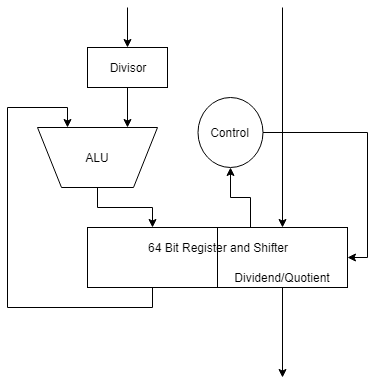
\includegraphics[width=.35\textwidth]{dividerDiagram.png}
    \caption{Design Diagram of Divider}
\end{figure}

\subsection*{Memory Elements}

All memory elements used in the processor are dflipflops except for two d latches used in the mult/div to latch onto the initial operation signal. From these, the processor utilizes 5 memory units which are referred to as stage latches. There is one for each F, D, X, M, and W. Their main implementation among them all is that they store whatever specific inputs they need to keep track and will output them at every positive clock edge. In doing so, the latches all remain synchronized to the clock and provide only one instruction per stage per cycle. This ensures that there aren't multiple operations occurring in the same stage in a single cycle.

\section*{Full Processor}

\subsection*{Pipeline}

As mentioned previously, the processor has 5 stages: Fetch, Decode, Execute, Memory, and Write. In implementation, these stages exist essentially as latches. For the fetch stage, it is the most simplest since it provides only the PC. It's inputs are either the sequentially next instruction (PC + 1) or a different value derived from a flow control instruction during its execution phase. The output of the fetch is fed to imem in order to fetch the full instruction from memory. For the decode latch, all it receives is the full instruction retrieved from ROM. Inside the latch, the instruction is stored to its registers and then broken up into Opcode, RD, RS, RT, shamt, ALU op, Immediate, and Target. These outputs may or may not be valid depending on the actual instruction from the Opcode, but the instruction is broken up into all possible formats regardless. Then during the decode stage, we decode the Opcode into the valid ISA instructions. With the specific instructions now defined, we then rearrange the fields to correctly reflect valid information of the instruction. For example, for a sw instruction, we copy RD to RT since eventually we need to read from both RD and RS and the processor will always read whatever is assigned to RS and RT. On the other hand, for a j instruction we do set RS and RT to zero to avoid accidental bypasses. Instructions will be further elaborated on later. For the execute stage, the latch takes in all the fields and instructions decoded previously. We do this to avoid re-decoding the instruction and opcode. Here, we perform any arithmetic for all the instructions that require it. This is also where flow control instructions will take into effect if their requirements are met. For memory stage, we get a smaller range of inputs, we don't need most of the fields or instructions that we decoded earlier anymore. Instead we maintain outputs from the alu, RD, if we're writing to memory, if we're writing to registers, and data to be written to memory. We are essentially left with all the information remaining that are completed in this stage or the next. Here we use the alu output if necessary to define an address in dmem and connect the data to be written to it also. If we are doing a sw instruction, the write enable will be asserted here. Otherwise, the pipeline continues into the final stage. Here we simply will write the output of the alu to registers as we've decoded an instruction that requires to do so in the previous stages.

\begin{figure}[htb!]
    \centering
    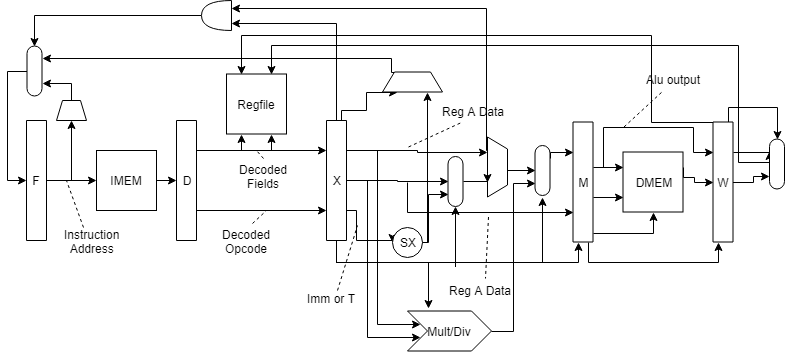
\includegraphics[width=.7\textwidth]{stageDiagram.png}
    \caption{Design Diagram for General Pipeline}
\end{figure}

\subsection*{Hazards}

Hazards are continuously checked by a hazard control unit and a bypass unit. In this implementation, one hazard that needs to be handled specifically with stalls are reads after writes. More specifically reading a register that a load will be writing to during the write stage. The data from a load is only available during the write stage, so if the following instruction needs it during the execute stage, then the instruction must be stalled. Formally, the processor stalls here if the opcode of the execute stage is for a load instruction and its RD equals either the RS or RT of the instruction in the decode stage; however, if it equals the RT and the instruction is a store, then we don't have to stall since there will be a bypass later on to handle this. We do the check here since it is the earliest possible time to be able to discern if a read after write will happen. Another hazard from this implementation is from a multiplication or division instruction. Since both operations require 32 cycles and they aren't pipelined, the processor must stall the instructions while the calculations are being performed.

\newpage

\begin{figure}[htb!]
    \centering
    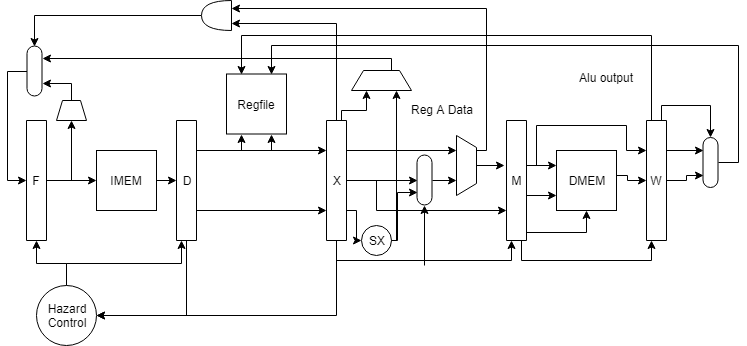
\includegraphics[width=.7\textwidth]{hazardDiagram.png}
    \caption{Design Diagram of Hazard Control Included}
\end{figure}

\subsection*{Bypassing}

Other than hazards that are stalled to be avoided, the processor will bypass data to avoid other potential hazards. The three bypasses are as follows: memory to execute, write to execute, and write to memory. For memory to execute, the intention is that sequential instructions that have a read after write can use data recently computed in the memory stage and bypass that into the execute stage in order to maintain the most recent value of a register being written to then read from. This goes for both RS and RT depending which ones match the RD for the memory stage. This is the same reasoning for write to execute. This is especially important since it is the reason why we only need to stall for one cycle instead of many for our hazard control. Once we can get data from a load, the latest we can bypass for most instructions is in execute. For the write to memory, we specifically need this bypass for a load word followed by a store word. This is the bypass that eliminates a stall instance mentioned earlier. Since store word doesn't need the actual register value of RT until memory, it can actually go through the pipe and get this bypass instead. RS matched the RD of write however, then the bypass doesn't help in this instance since we still need to add the offset.

\begin{figure}[htb!]
    \centering
    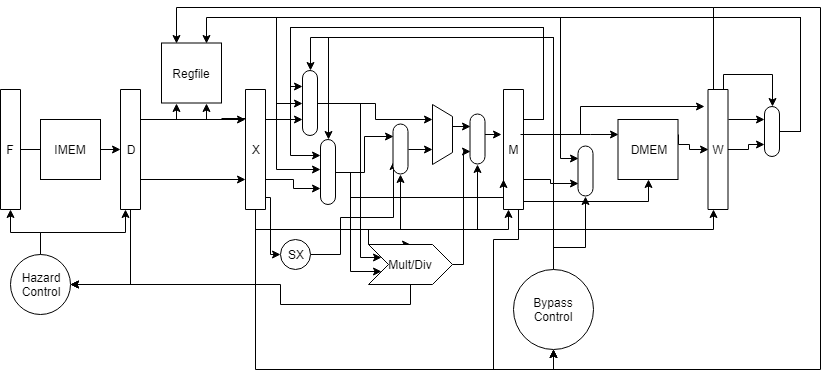
\includegraphics[width=.7\textwidth]{bypassDiagram.png}
    \caption{Design Diagram of Bypass Control Included}
\end{figure}

\subsection*{Efficiency}

The fastest that the processor has been clocked is roughly 68 MHz. Overall the efficiency is moderate. There can be stalls due to the load read after write hazard which can be resoled if we possibly add in a second ALU in the memory stage which we prevent the stall but we drastically increase area usage and idle component if we were to use it only for read after writes from loads. Also since our mult/div is 32 cycles long, having a second alu that could potentially perform this operation would mean we have to stall an extra stage in the event that the memory alu needs to run. In this manner, the one stall is a hit that is optimal given the stages we used to implement. As mentioned, our mult/div is pretty inefficient compared to the rest of the processor. It takes a full 32 cycles to complete and it doesn't pipeline sequential mult/div operations. In the end, this means every mult/div operation costs us 32 cycles. If mult/div was pipelined, we could save a $32(n-1)$ cycles for $n$ sequential mult/div instructions. In addition to pipelining, there are possible other multiplication algorithms to decrease the required number of cycles to perform a single multiplication. For example modified Booth's would half the number of cycles needed. Other than the two points mentioned, the processor is able to perform a majority of combinations of instructions without needing extra stalls.

\section*{Instruction Implementation}

\subsection*{R-Type Instructions}

All R-Type instructions were fairly straightforward to implement in the processor. Given that the ALU provided functions properly and already implements all of the operations except for mult/div, the only implementation detail was correctly providing fields extracted from the instruction and watching out for hazards. Any R-type instruction is first formatted during the decode stage. Here, the processor doesn't have to do any changes to RD, RS, or RT since all three fields are used in the operation as specified by the format. Other important fields such as ALU op code and shift amount have already been decoded and since the Opcode specifies a R-Type, we will actually end up using these fields. In the execute stage we simply feed all the parameters to the ALU or mult/div. Mult/div in the processor is not a submodule within the ALU, but is instead its own discrete module. It functions in parallel with the ALU, but it can start the stalling chain if the ALU op code specifies a multiply or divide instruction. Otherwise, the processor will then save the output of either the AlU or mult/div to the M latch. Nothing is done in this stage and the output continues to the write stage. Here, all R-type instructions will write to a register so we have the write register bit enabled and write to RD that we persisted since the decode stage. As mentioned in previous parts, there are specific bypasses and stalls that may occur and are detected by comparing the RS and RT of the R-type instruction with the Rd of earlier instructions in the pipeline.

\subsection*{I-Type Instructions}

I-Type instructions generally follow a similar flow of logic and slight adjustments from R-type instructions. Again, it's straightforward for all instructions up to the decode stage. Here, we have to do some reaaranging with register addresses we're reading from. For I-type instructions we will always read for RS, but we may sometimes read from RD. The only instruction that doesn't necessarily need to read from RD is load, which we go ahead and set RT to 0 then. Continuing into execute stage, we set the ALU op code to 00000 since every I-Type instructions either needs to add or compare values. Again, we need to be careful with what we input to the ALU. In the processor, operand A is set to whatever we got from register RS. For operand B we have the following options: Imm (N) for addi, sw, and lw; and RT for bne and blt. For the former case, this output is used to address a space in DMEM or is destined to be saved in a register which will follow down the pipeline as expected whhere sw and lw will take into effect in memory and addi will occur in write. For bne and blt, we signal that a jump is to occur. While the ALU was comparing the values, a separate adder is used to add the PC + 1 stored with the instruction and the Imm value. If the conditions are met, a branch boolean is signaled causing the processor to flush out the fetch stage and decode stage and setting the PC to the output of the adder. Afterwards, bne and blt will continue down the pipeline and not do anything during those stages since there is no remaining logic to be done.

\subsection*{JI-Type Instructions}

For the 350 ISA, there are 4 total JI-type instructions. The most simplest and straightforward instruction is j.All read registers, RS and RT, are both set to 0. The j instruction makes its way to the execute stage where the branch boolean is again asserted to flush out instructions and prepare to change PC to the lower 12 bits of the T field. Afterwards, similar to bne and blt, the j instruction will continue through the pipe and make no more changes. For jal and setx, the RD is hard coded during the decode stage to direct to \$31 and \$30 respectively according to the ISA. Then no additional computations are required in the execute stage. The only change here, is instead of outputting the ALU results, we instead will output either PC + 1 (which has been padded with leading 0's to be 32 bits wide) or T (which has been sign extended). For jal, it will perform exactly like j with its branch flow logic. The key difference here, is that these two instructions will continue to the write stage and will write the corresponding information into their specified registers set earlier in the decode stage. The last remaining JI-type instruction is bex. Here we hard code in the decode stage to set RS to point to \$30. In the execute stage we set operand A to the ALU to be whatever we read for RS and set operand B to be 0. If this condition holds true, we essentially perform the same operation as j. Either way, bex does nothing else in the pipe and will exit quietly throught the rest of the stages.

\subsection*{JII-Type Instructions}

There is only one JII-type instruction in the ECE 350 ISA and it is jr. This is pretty much the opposite of jal. Instead of RD being set to \$31, we set RS to \$31. In execute, we take the lowest 12 bits of the output from the regfile and set this as the next PC address. Again, jr will then continue peacefully out of the pipeline.

\section*{Process}

Most of the implementation choices I made were based of the specifications of the project and familiarity with design options from the course lectures. The five staged pipeline with latches were from the project spec sheet. All of the bypasses and stall logic were learned from the course and reference materials. The mult/div and adder were also derived from concepts taught in the course. The personal choices I made was how instruction information persisted through the pipeline. As shown, I broke up the information early. This choice came out of avoiding to compute the decode function several times throughout the pipeline and instead do it once and reserve more registers to preserve the decoded information. Along with that, the mult/div implementation choice was simply to get instructions working soon as possible. I am aware of ways to improve this implementation as described previously, but ultimately the design currently works and does not have too much of a drastic impact on the processor as a whole.

To test out the processor throughout the implementation phase, I created a testbench that would provide a clock to the processor and set up probes into wires within various submodules. This testbench allowed me to make sure that expected values were being stored or communicated throughout the processor. It also allowed me to see what was going on at every stage of the pipeline. In addition to the test bench, I wrote simple MIPS programs and used the ECE 350 assembler to convert the file into a .mif file for the processor to read from. For gate timing analysis, I made specific outputs for the processor that mimicked the wires I also monitored in the test bench. Then I used a waveform to provide a clock and checked all the specific outputs I made for expected values throughout the pipe.

The only errors that currently exist in the processor are exceptions for multiplication operations. Specifically,  the processor doesn't detect it and handle exceptions raised by the mulitplication part of mult/div properly. The error occurred when I was testing the exceptions for the arithmetic instructions and mult was the only one that didn't follow expected outcomes. To test it, I outputted more related wires with a mult operation to see what is going on in a waveform. It appears that the exception flag is not raised, but the mult/div was working fine with a testbench testing for exception handling. Given more time, I would revisit the logic in handling multiplication exceptions and make sure this flag becomes a more stable output for the multdiv.

The biggest challenges to this project involved getting timings correct so that the pipeline would function as intended. In one case, it was discovering that Quartus defaults the ROM and RAM to have registered inputs and outputs. For a lot of the project I was dealing with extremely delayed results from IMEM and DMEM. At first when I discovered this significant delay, I chose to bypass the latches that read from their outputs (D and W). Due to the bypassing, D had an extreme amount of extra logic to it to ensure that it provided stable outputs within a clock cycle. During the last few days, it was brought to my attention that I could remove the registered outputs and instead the outputs would be available in half the time as before. At that point, was able to revert the D and W latch back to simple registers without any special bypass logic. Another challenge related to timing that I faced was resolving what areas of the pipeline were throttling the processor as a whole. Ultimately I had to refactor some of my wiring to remove multiple leveled ternary operators so that some comparisons would occur in parallel to decrease the amount of time it took to get the desired result.

The main learning point I took away from making this processor is that if timing is an issue, there is probably a way to sacrifice area for increased performance. In the scope of this class, it is often better to do so and take the tradeoff of shorter costs for larger area. Also, as I mentioned in the challenges part, another takeaway from this project was being to be conscious that verilog feels like a coding language, but specific ways of coding it can provide better timings to other alternatives. For me, this was when I broke up a chained ternary operation into several independent ternary operations that either outputted a specific value or would be just high impedance.

\section*{Conclusion}

Given the specifications of the project checkpoint and ISA to implement, I have created a 5 staged processor that has hardware interlocks built in. By incorporating memory modules, register files, ALU, and mult/div module the processor is able to handle a variety of arithmetic operations and flow logic operations. The overall design is efficient in handling data hazards with minimal cycle waste. The only area of improvement would be implementing a better multiplication algorithm and redesigning mult/div to be able to be pipelined. Alternatively additional instructions could be incorporated into the ISA to provide other operations besides the instructions currently implemented. This could involve I/O instructions to interface with the module for a larger range of applications.

\end{document}